\og \emph{Dans un triangle non équilatéral, la droite d'Euler est la droite qui passe par les trois points suivants }:

	\begin{itemize}[itemsep=0pt]
		\item \emph{le centre du cercle circonscrit à ce triangle (cercle passant par les trois sommets de ce triangle).}
		\item \emph{le centre de gravité de ce triangle situé à l'intersection des médianes de ce triangle.}
		\item \emph{l'orthocentre de ce triangle situé à l'intersection des hauteurs de ce triangle \fg{}}.
	\end{itemize}

	\begin{minipage}[t]{0.5\linewidth}
		Le but de l'exercice est d'étudier un exemple de droite d'Euler.

	On considère un cube ABCDEFGH de côté une unité.

	L'espace est muni du repère orthonormé $\left(\mathrm{A} ~;~ \vectt{AB} ~;~ \vectt{AD} ~;~ \vectt{AE}\right)$.

	On note I le milieu du segment [AB] et J le milieu du segment [BG].
	\end{minipage}
	\hfill
	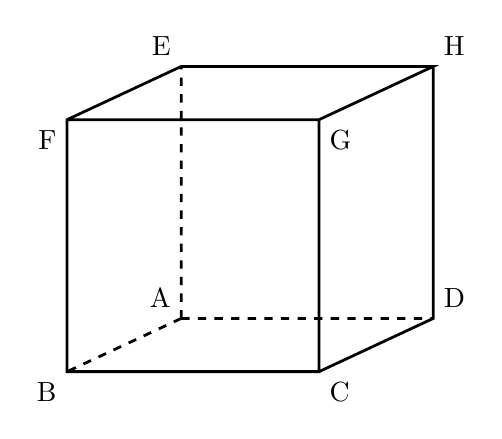
\begin{tikzpicture}[x=(205:16mm),y=(0:32mm),z=(90:32mm),baseline={(E.base)}]
		\draw [line width=1pt]
		(1,0,0)node[below left]{B}--
		(1,1,0)node[below right]{C}--
		(1,1,1)node[below right]{G}--
		(0,1,1)node[above right]{H}--
		(0,0,1)node[above left](E){E}--
		(1,0,1)node[below left]{F}--cycle
		(1,0,1) --(1,1,1) (1,1,0)--(0,1,0)--(0,1,1);
		\draw[line width=1pt,dashed] (0,0,0)node[above left]{A}--(0,1,0)node[above right]{D}
		(0,0,0) -- (1,0,0) (0,0,0)--(0,0,1);
	\end{tikzpicture}

	\begin{enumerate}
		\item Donner sans justification les coordonnées des points A, B, G, I et J.

		\item \begin{enumerate}
			\item Déterminer une représentation paramétrique de la droite (AJ).

			\item Montrer qu'une représentation paramétrique de la droite (IG) est : \[\left\{\begin{array}{l}x=\dfrac{1}{2}+\dfrac{1}{2} t \\ y=\phantom{\dfrac{1}{2}+\dfrac{1}{2}}t \\ z=\phantom{\dfrac{1}{2}+\dfrac{1}{2}}t\end{array} \right.\quad\text{ avec }t \in \R.\]

			\item Démontrer que les droites (AJ) et (IG) sont sécantes en un point S de coordonnées S$\left(\dfrac{2}{3} ~;~ \dfrac{1}{3} ~;~ \dfrac{1}{3}\right)$.
		\end{enumerate}

		\item \begin{enumerate}
			\item Montrer que le vecteur $\vect{n}(0 ~;~-1 ~;~ 1)$ est normal au plan (ABG).

			\item En déduire une équation cartésienne du plan (ABG).

			\item On admet qu'une représentation paramétrique de la droite $(d)$ de vecteur directeur $\vect{n}$ et passant par le point K de coordonnées $\left(\dfrac{1}{2} ~;~ 0 ~;~ 1\right)$ est : \[\left\{\begin{array}{l}
x=\dfrac{1}{2} \\
 y= \phantom{\dfrac{1}{2}}- t \\
  z=1+t\end{array} \right.\quad\text{ avec }t \in \R.\]

			Montrer que cette droite $(d)$ coupe le plan (ABG) en un point L de coordonnées L$\left(\dfrac{1}{2} ~;~ \dfrac{1}{2} ~;~ \dfrac{1}{2}\right)$.

			\item Montrer que le point L est équidistant des points A, B et G.
		\end{enumerate}

		\item Montrer que le triangle ABG est rectangle en B.

		\item \begin{enumerate}
			\item Identifier le centre du cercle circonscrit, le centre de gravité et l'orthocentre du triangle ABG (aucune justification n'est attendue).

			\item Vérifier par un calcul que ces trois points sont effectivement alignés.
		\end{enumerate}
	\end{enumerate}
